\documentclass{assignment}

\course{ECO 120-04}
\name{Lucas Reddinger}
\date{Wednesday 23 November 2022}
\doctitle{Assignment 10: Stagflation}

\begin{document}
\RaggedRight

\beginassignment{}

\emph{Due Monday 28 November.} Please submit hardcopy at the beginning of class (11:00 a.m.), or if you prefer, under the door of Wimberly Hall 339C by 10:50 a.m.

\ornamentalrule

Suppose that the U.S.~economy is initially in long-run equilibrium, producing its potential output $Y_P$, as depicted directly below.

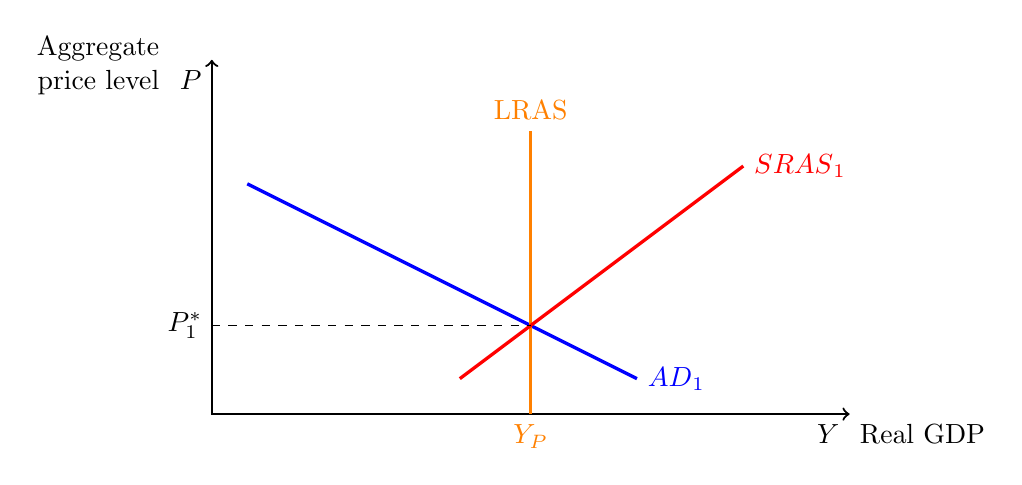
\begin{tikzpicture}[scale=0.45]
\draw[thick,<->] (0,10) node[below left,label={[align=right]left:Aggregate\\price level\\ }] {$P$} --(0,0)--(18,0) node[below left,label=right:Real GDP]{$Y$};
\draw[very thick,blue] (1,6.5) --(12,1) node[right]{$\text{AD}_1$};
\draw[very thick,orange] (9,0) node[below]{$Y_P$}--(9,8) node[above]{LRAS};
\draw[very thick,red] (7,1)--(15,7) node[right]{$\text{SRAS}_1$};
\draw[dashed] (0,2.5) node[left]{$P^*_1$} --(9,2.5) ;
\end{tikzpicture}

A multinational effort to sanction Russian oil and natural gas results in a negative shock to short-run aggregate supply from $\text{SRAS}_1$ to $\text{SRAS}_2$ as depicted below. U.S.~economic output falls from $Y_P$ to $Y^*_2$, and the aggregate price level rises from $P^*_1$ to $P^*_2$. This results in a period of \emph{stagflation}---lower economic output coupled with inflation.

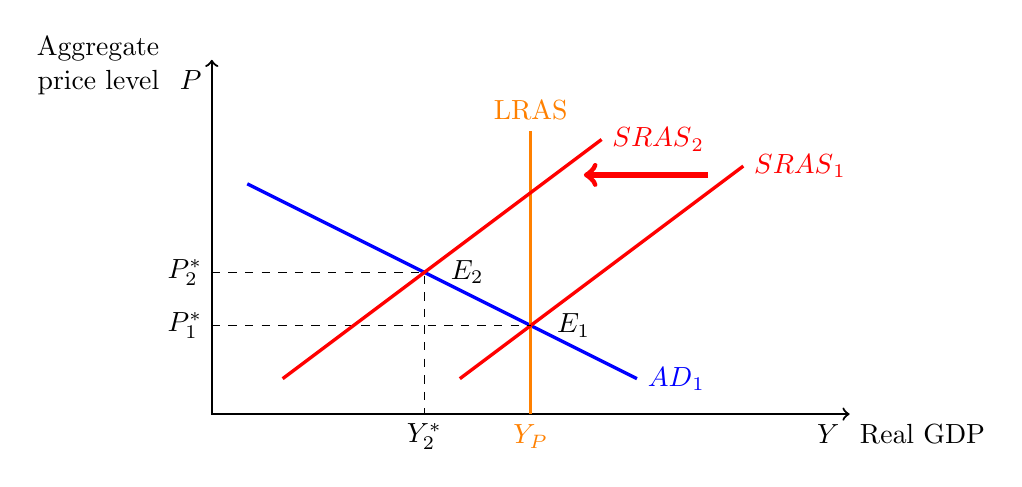
\begin{tikzpicture}[scale=0.45]
\draw[thick,<->] (0,10) node[below left,label={[align=right]left:Aggregate\\price level\\ }] {$P$} --(0,0)--(18,0) node[below left,label=right:Real GDP]{$Y$};
\draw[very thick,blue] (1,6.5) --(12,1) node[right]{$\text{AD}_1$};
\draw[very thick,orange] (9,0) node[below]{$Y_P$}--(9,8) node[above]{LRAS};
\draw[very thick,red] (7,1)--(15,7) node[right]{$\text{SRAS}_1$};
\draw[dashed] (0,2.5) node[left]{$P^*_1$} --(9,2.5) node[right,xshift=6pt]{$E_1$};
\draw[very thick,red] (2,1) --(11,7.75) node[right]{$\text{SRAS}_2$};
\draw[dashed] (0,4) node[left]{$P^*_2$} --(6,4) node[right,xshift=6pt]{$E_2$} --(6,0)node[below]{$Y^*_2$};
\draw[line width=2pt,->,red] (14,6.75)--(10.5,6.75);
\end{tikzpicture}


\begin{enumerate}

\item \label{maintain-output} Please illustrate how fiscal policy could be used to maintain economic growth. \\ {\footnotesize Hint: Reproduce the second graph here. Illustrate a change in fiscal policy that restores output to $Y_P$.}

\vfill

\item \label{maintain-prices} Please illustrate how fiscal policy could be used to stabilize prices. \\ {\footnotesize Hint: Reproduce the second graph here. Illustrate a change in fiscal policy that restores the price level to $P^*_1$.}

\vfill

\item Can fiscal policy remedy stagflation? Please explain with a complete sentence.  \\ {\footnotesize Hint: Can a change in fiscal policy restore \emph{both} output to $Y_P$ \emph{and} the price level to $P^*_1$?}

\vspace{2\baselineskip}

\end{enumerate}

\end{document}
